\chapter{Type Inference}
\begin{figure}[htbp]
   \centering
   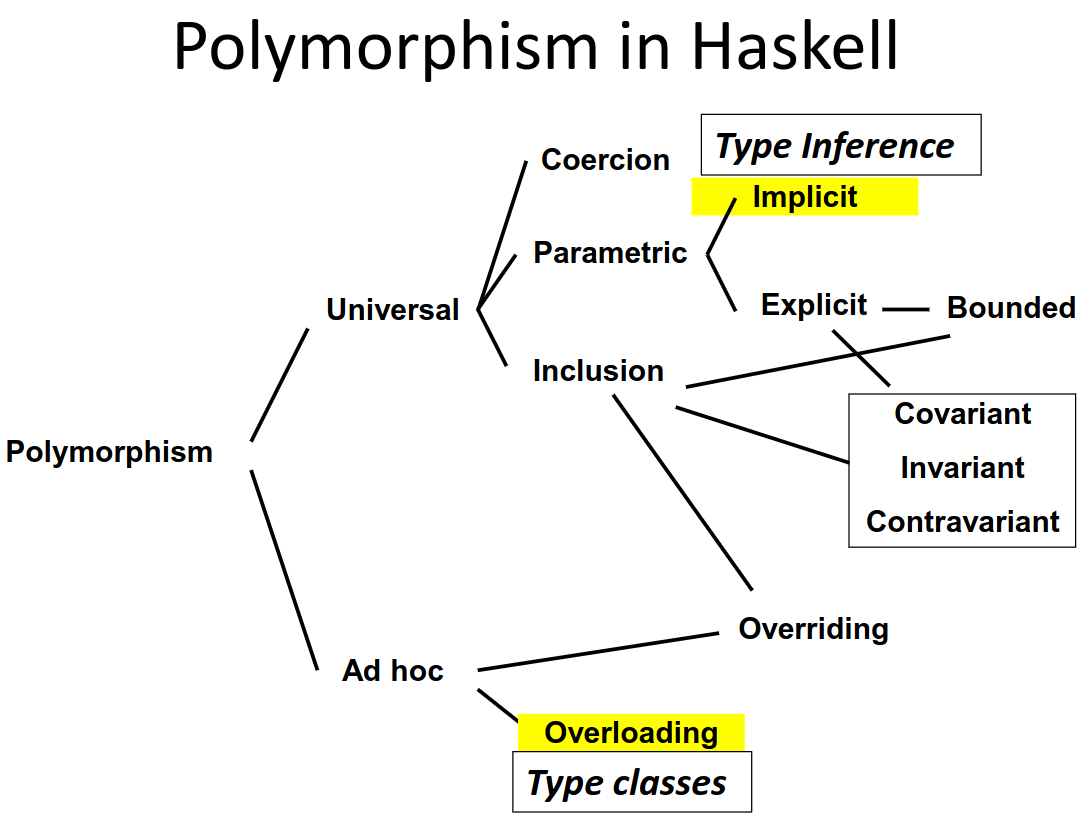
\includegraphics{images/haskell_polymorphism.png}
   \caption{Haskell Polymorphism Recap}
   \label{fig:haskell_polymorphism}
\end{figure}

\section{Overloading}
Haskell allows \textbf{overloading} even of \textbf{primitive types}:
the code to be executed is determined by the type of the arguments,
leading to have \textit{early binding} in \textit{statically} typed languages
or \textit{late binding} in \textit{dynamically} typed languages.

In Haskell we can write the following, but what is the type? May be float, int, double, etc.
\begin{lstlisting}
   sqr x = x * x
\end{lstlisting}

\note{
   \tiny
   Actually in Haskell, we have \ul{type classes}
   \texttt{sqr :: Num a => a -> a}
}

When considering overloading besides arithmetic, we find that some functions are \textbf{fully polymorphic}:
\begin{lstlisting}
   length :: [w] -> Int
\end{lstlisting}

While others not so much;
for example, \textit{membership} works only for types that support equality,
while \textit{sorting} works only for types which support \textit{ordering}. 
\begin{lstlisting}
   member :: [w] -> w -> Bool
   sort :: [w] -> [w]
\end{lstlisting}

\section{Type Classes}
\textbf{Type Classes} solve many overloading problems concerning arithmetic and equality (and similar properties) support.

The idea is to generalize ML’s eqtypes to arbitrary types
and provide concise types to describe overloaded
functions, so no exponential blow-up (i.e. defining functions for every possible combination of type arguments).\\
Type classes allow users to define functions using overloaded
operations {---}e.g. square, squares, and member{---} and to
declare new collections of
overloaded functions: equality and arithmetic
operators are not privileged built-ins.
Haskell's solutions fits perfectly within type inference framework.

The intuition is that a sorting function may allow to be passed a comparison \lstinline|cmp| operator as argument,
thus making the function parametric, instead of having it rely on overloaded operators.
\begin{lstlisting}
   qsort:: (a -> a -> Bool) -> [a] -> [a]
   qsort cmp [] = []
   qsort cmp (x:xs) = qsort cmp (filter (cmp x) xs) ++ [x] ++
   qsort cmp (filter (not.cmp x) xs)
\end{lstlisting}

Developing this idea, consider rewriting the parabola function to take operators as argument
\begin{lstlisting}
   parabola x = (x * x) + x
   parabola' (plus, times) x = plus (times x x) x
\end{lstlisting}
Here the extra parameter is a \textit{\textbf{dictionary}} that provides implementations for the overloaded ops.
These implies rewriting calls to pass appropriate implementations for plus and times:
\begin{lstlisting}
   y = parabola'(intPlus,intTimes) 10
   z = parabola'(floatPlus, floatTimes) 3.14
\end{lstlisting}

There's more, let's try to actually define such dictionary along with getters to get the appropriate implementation.
\begin{lstlisting}
   -- Dictionary type
   data NumDict a = MkNumDict (a->a->a) (a->a->a)
   -- Accessor functions
   get times :: NumDict a -> (a->a->a)
   get times (MkNumDict times plus) = times
   get plus :: NumDict a -> (a->a->a)
   get plus (MkNumDict times plus) = plus
\end{lstlisting}

Hence we can define the parabola function to take a dictionary as argument, and we can call it passing to a dictionary of the appropriate type.
\begin{lstlisting}
   -- Dictionary-passing style
   poly2 :: NumDict a -> a -> a
   poly2 dict x = let times = get times dict
         plus = get plus dict
      in times x (plus x x)

   -- Dictionary creation
   intDict = MkNumDict int times int plus
   floatDict = MkNumDict float times float plus

   -- Passing dictionaries
   y = poly2 intDict 10
   z = poly2 floatDict 2.71
\end{lstlisting}
The function \lstinline|poly2| is a polymorphic function that provides the desired behavior
of the overloaded function poly.
Of course, this series of transformations would be tedious for a programmer
to carry out. To avoid this tedium, Haskell’s type class mechanism automates the
rewriting process, as we will see in the following sections.


Consider that the type class mechanism in Haskell is made of comprised of three components: type class
declarations, type class instance declarations, and qualified types.
\begin{enumerate}
   \item \textbf{Type class declarations}
   \begin{enumerate}
      \item Define a set of operations and give it a name
      \item Example: \lstinline|Eq a| type class
      \begin{itemize}
      	\item operations \lstinline|==| and \lstinline|\=| with \lstinline|type a -> a -> Bool|
      \end{itemize}
      \begin{lstlisting}
         class Num a where
         (*) :: a -> a -> a
         (+) :: a -> a -> a
         negate :: a -> a
         ... <other numeric operations> ...
      \end{lstlisting}
   \end{enumerate}
   \item \textbf{Type class instance declarations}
   \begin{enumerate}
      \item Specify the implementations for a particular type
      \item For \lstinline|Int| instance, \lstinline|==| is defined to be integer equality
   \end{enumerate}
   \begin{lstlisting}
         instance Num Int where
         (*) = int_times
         (+) = int_plus
         negate x = int_negate x
         ... <other numeric operations> ...

         instance Eq Int where
            i == j = int eq i j
            i /= j = not (int eq i j
   \end{lstlisting}
   \item \textbf{Qualified types} (or Type Constraints)
   Concisely express the operations required \st{on otherwise polymorphic type} to convert an overloaded
   function into a polymorphic one.\\
   The \lstinline|Eq t =>| prefix of this type is what makes it qualified.
   \begin{lstlisting}
      member:: Eq w => w -> [w] -> Bool
      double :: Num t => t -> t
      poly :: Num t => t -> t
   \end{lstlisting}
   If a function is \textit{not} qualified, then \ul{it must be purely polymorphic and work for any type whatsoever.}
\end{enumerate}

So, considering our previous examples, the type of \lstinline|member| parameters is any type \lstinline|w| that supports equality, i.e. that belongs to the \lstinline|Eq| type class.
\lstinline|reverse| instead, works for any list of any type.
\begin{lstlisting}
   member :: Eq w => w -> [w] -> Bool
   sort :: Ord w => [w] -> [w]
   reverse :: [w] -> [w]
\end{lstlisting}

\labelitemize{
   \textit{implementation summary}
}{
   \begin{enumerate}
      \item Each overloaded symbol has to be introduced in at least one type class
      \item The compiler translates each function that uses an overloaded symbol into a function with an extra parameter: the dictionary.
      \item References to overloaded symbols are rewritten by the compiler to lookup the symbol in the dictionary.
      \item The compiler converts each type class declaration into a dictionary type declaration and a set of selector functions.
      \item The compiler converts each instance declaration into a dictionary of the appropriate type.
      \item The compiler rewrites calls to overloaded functions to pass a dictionary. It uses the static, qualified type of the function to select the dictionary.
   \end{enumerate}
}

\subsection{Compositionality}
\textbf{Compositionality} in type classes refers to the ability to \ul{combine and reuse type classes to build more complex abstractions}, allowing to define new type classes that inherit functionalities from existing ones.

You can define new type classes that combine multiple existing ones. For example, you might create a \lstinline|ShowRead| type class that requires both \lstinline|Show| and \lstinline|Read| instances, enabling both string conversion and parsing
\begin{lstlisting}
   class (Show a, Read a) => ShowRead a where
      showRead :: a -> String
      showRead x = show x ++ " " ++ show (read (show x) :: a)

\end{lstlisting}


This also applies to type classes instance declarations.
When you declare an instance for a type, you can combine multiple type classes to ensure that the type satisfies all the required constraints. For example, if you have a type that needs to be both \lstinline|Eq| and \lstinline|Show|, or you have two types which need to be both \lstinline|Eq| as in the example below, you can declare an instance for both type classes at once.
\begin{lstlisting}
   class Eq a where
   (==) :: a -> a -> Bool
   instance Eq Int where
   (==) = intEq -- intEq primitive equality
   instance (Eq a, Eq b) => Eq(a,b) where
   (u,v) == (x,y) = (u == x) && (v == y)
   instance Eq a => Eq [a] where
   (==) [] [] = True
   (==) (x:xs) (y:ys) = x==y && xs == ys
   (==) _ _ = False
\end{lstlisting}

\subsection{Compound Translation}
\newpage
\subsection{Subclasses}
\begin{paracol}{2}
   \vspace{\fill}
   \begin{lstlisting}[label={lst:hs_eqnum}]
      memsq :: (Eq a, Num a) => a -> [a] -> Bool
      memsq x xs = member (square x) xs
   \end{lstlisting}
   We could treat the Eq and Num type classes separately as in \ref{lst:hs_eqnum}, but we expect that every instance of Num is also an instance of Eq.
   A subclass declaration expresses this relationship:
   \begin{lstlisting}
      class Eq a => Num a where
      (+) :: a -> a -> a
      (*) :: a -> a -> a
   \end{lstlisting}
• With that declaration, we can simplify the type of the function

\begin{lstlisting}
   memsq :: (Eq a, Num a) => a -> [a] -> Bool
   memsq x xs = member (square x) xs
\end{lstlisting}

\vspace{\fill}
\switchcolumn

\begin{figure}[htbp]
   \centering
   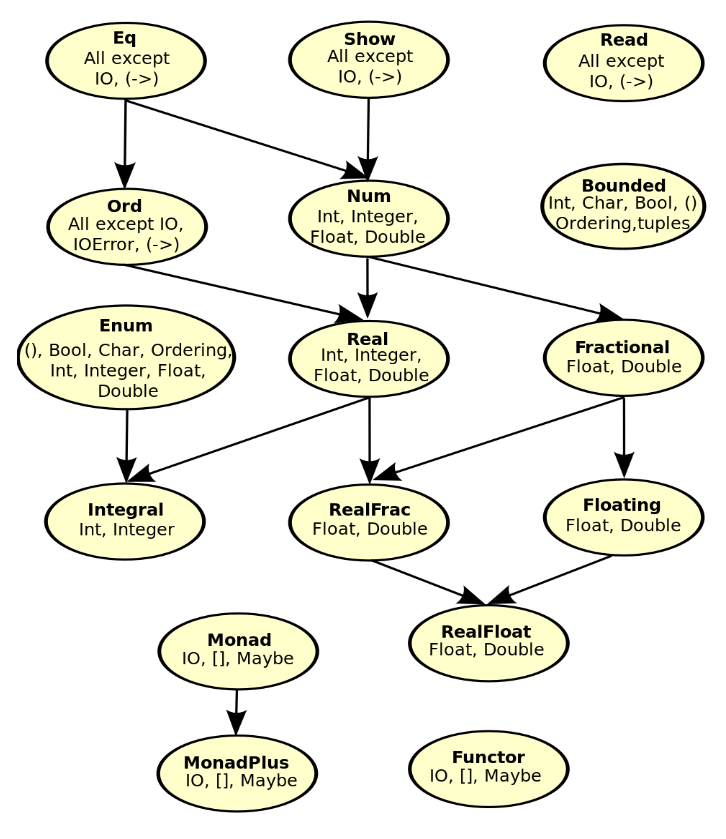
\includegraphics{images/haskell_subclasses.png}
   \caption{Haskell Subclasses relationships}
   \label{fig:haskell_subclasses}
\end{figure}

\end{paracol}

\subsection{Deriving}
For Read, Show, Bounded, Enum, Eq, and Ord, the compiler
can generate instance declarations automatically.
\begin{lstlisting}
   data Color = Red | Green | Blue
      deriving (Show, Read, Eq, Ord)
   
   Main>:t show
   show :: Show a => a -> String
   Main> show Red
   "Red"
   Main> Red < Green
   True
   Main>:t read
   read :: Read a => String -> a
   Main> let c :: Color = read "Red"
   Main> c
   Red
\end{lstlisting}

\subsection{Numeric Literals}
\begin{lstlisting}
   class Num a where
      (+) :: a -> a -> a
      (-) :: a -> a -> a
      fromInteger :: Integer -> a
      -- Even literals are overloaded.
      -- 1 :: (Num a) => a
      ...

   inc :: Num a => a -> a
   inc x = x + 1
\end{lstlisting}

\labelitemize{
   \textit{Advantages}
}{
   \setlength{\leftskip}{1em}
   Numeric literals can be interpreted as values of any
   appropriate numeric type,
   for example: 1 can be an Integer or a Float or a user-
   defined numeric type.
}

\subsection{Missing Notes}
Look at slides $34...64$ for more on Type Inference.

\section{Inferencing types}
In standard type checking the compiler examine body of each function and uses declared types to check agreement;
type inference instead consists in examining code without type information, and infer the
most general types that could have been declared

\subsection{Steps schematics}
\begin{figure}[htbp]
   \centering
   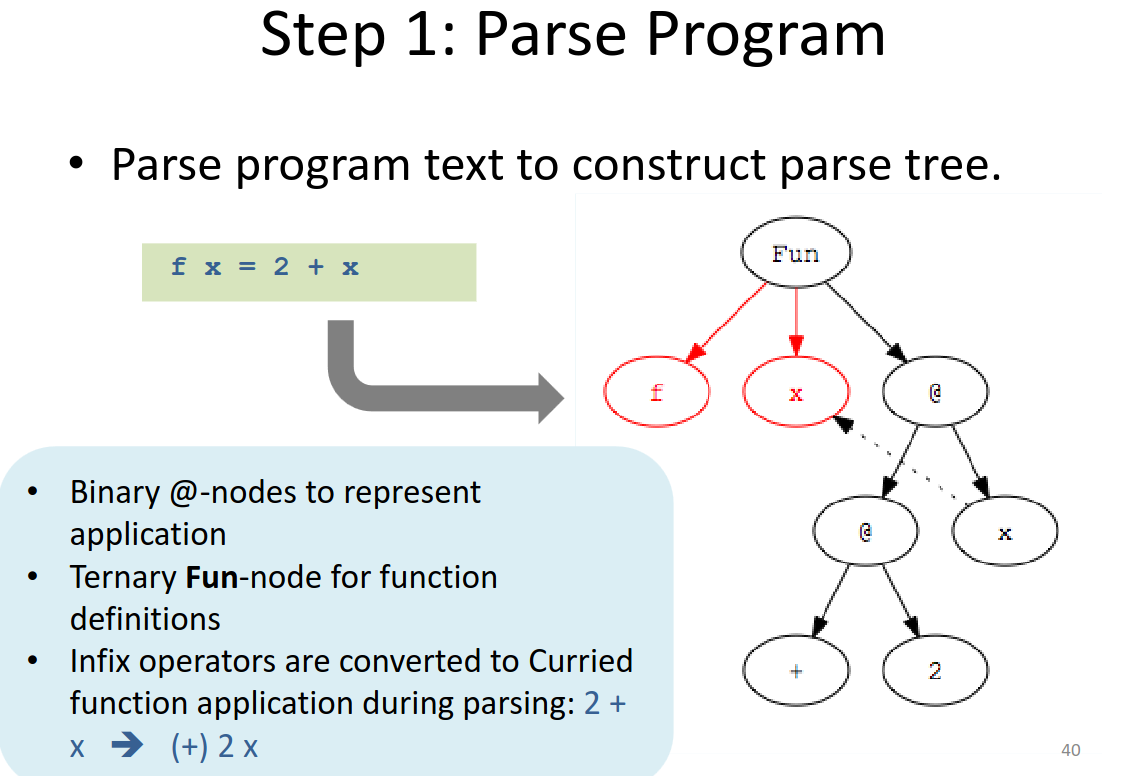
\includegraphics[width=0.4\columnwidth]{images/typeinference_step1.png}
   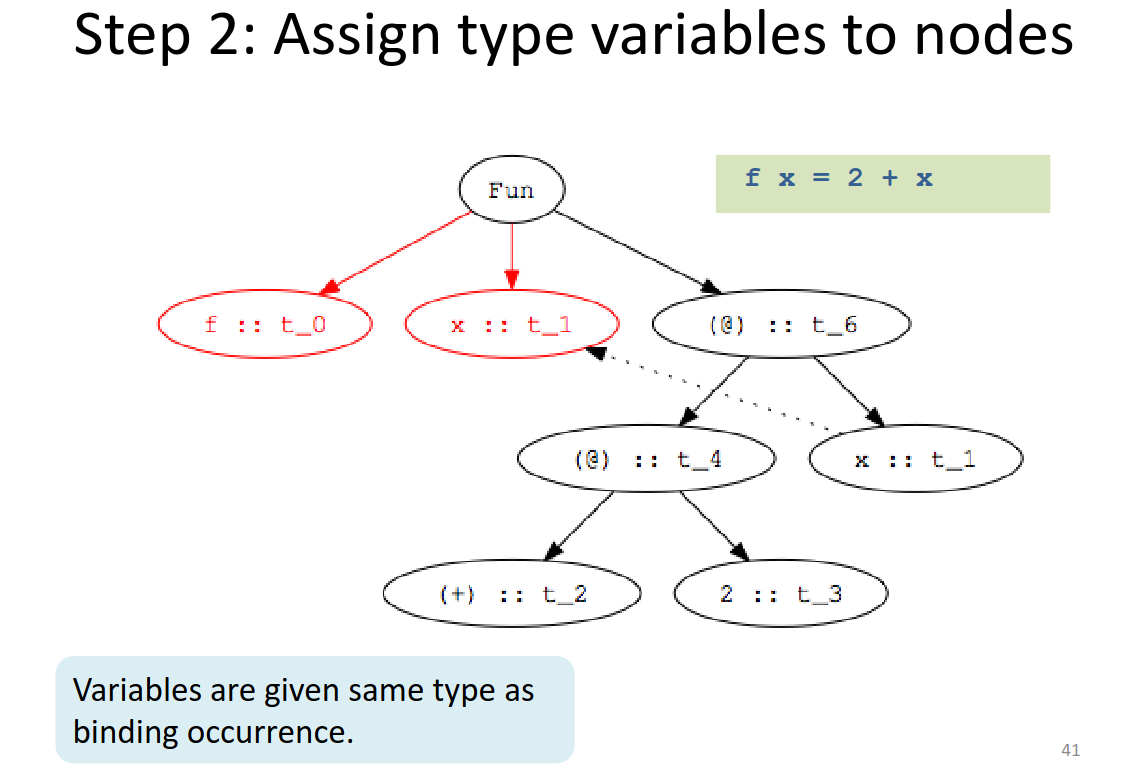
\includegraphics[width=0.4\columnwidth]{images/typeinference_step2.png}
   \label{fig:typeinference_step1_2}
\end{figure}

% \begin{figure}[htbp]
%    \centering
%    \label{fig:typeinference_step2}
% \end{figure}

\textbf{Constraints} can be deduced from (function) \textit{Application} nodes \lstinline|f x| and from \textit{Abstractions} \lstinline|f x = e|.

\begin{figure}[htbp]
   \centering
   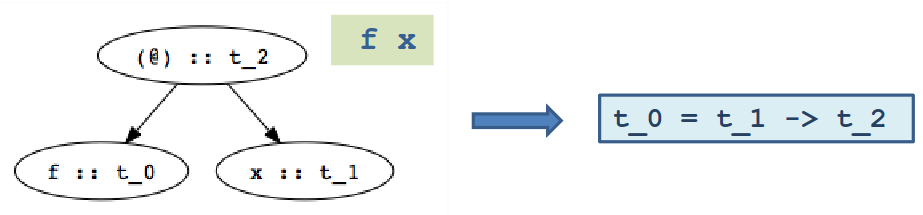
\includegraphics{images/typeinference_constraints_application.png}
   \caption{Deducing constraints from function application}
   \label{fig:typeinference_constraints_application}
\end{figure}
\begin{itemize}
   \item Type of \lstinline|f| (\lstinline|t_0| in figure) must be $domain \longrightarrow range$.
   \item \textbf{Domain} of \lstinline|f| must be type of argument \lstinline|x| (\lstinline|t_1|)
   \item \textbf{Range} of f must be result of application (\lstinline|t_2|)
   \item \textbf{Constraint}: \lstinline|t_0 = t_1 -> t_2|
\end{itemize}

\begin{figure}[htbp]
   \centering
   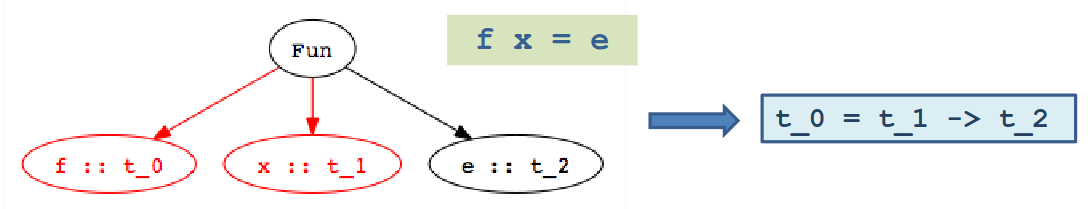
\includegraphics{images/typeinference_constraints_abstraction.png}
   \caption{Deducing constraints from abstractions}
   \label{fig:typeinference_constraints_abstraction}
\end{figure}


\begin{figure}[htbp]
   \centering
   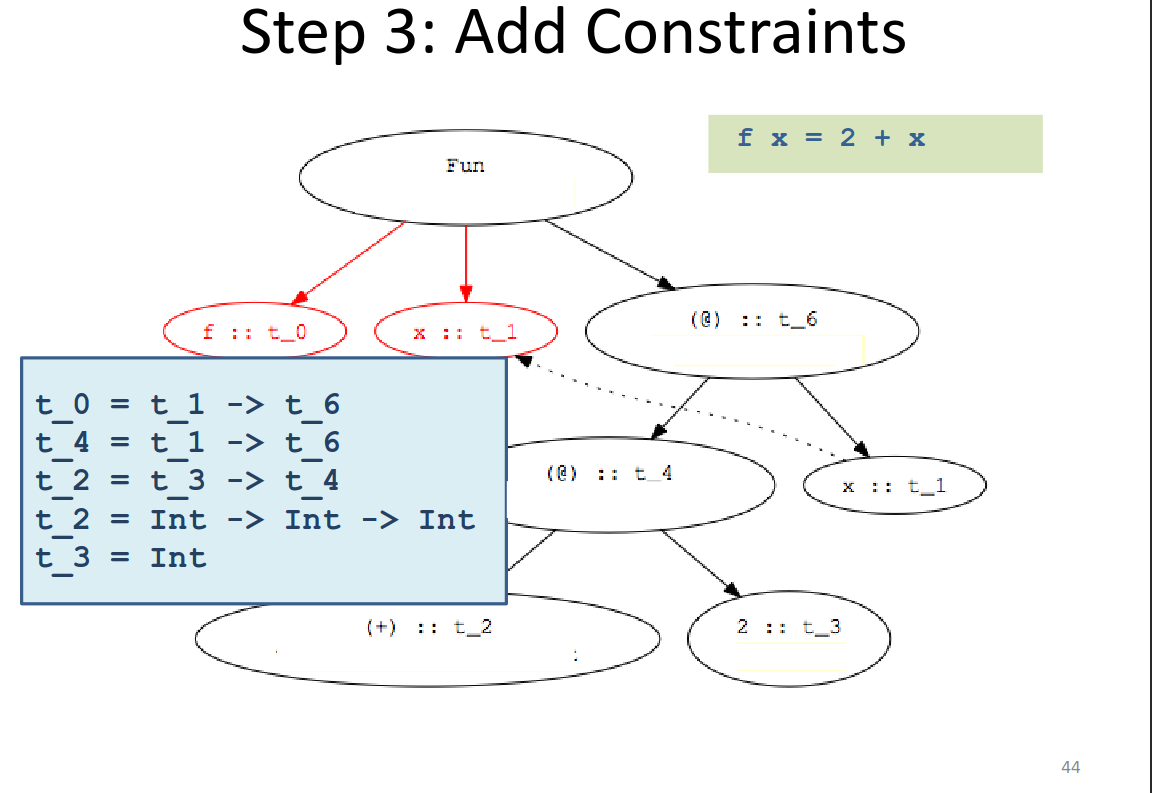
\includegraphics[width=0.4\columnwidth]{images/typeinference_step3.png}
   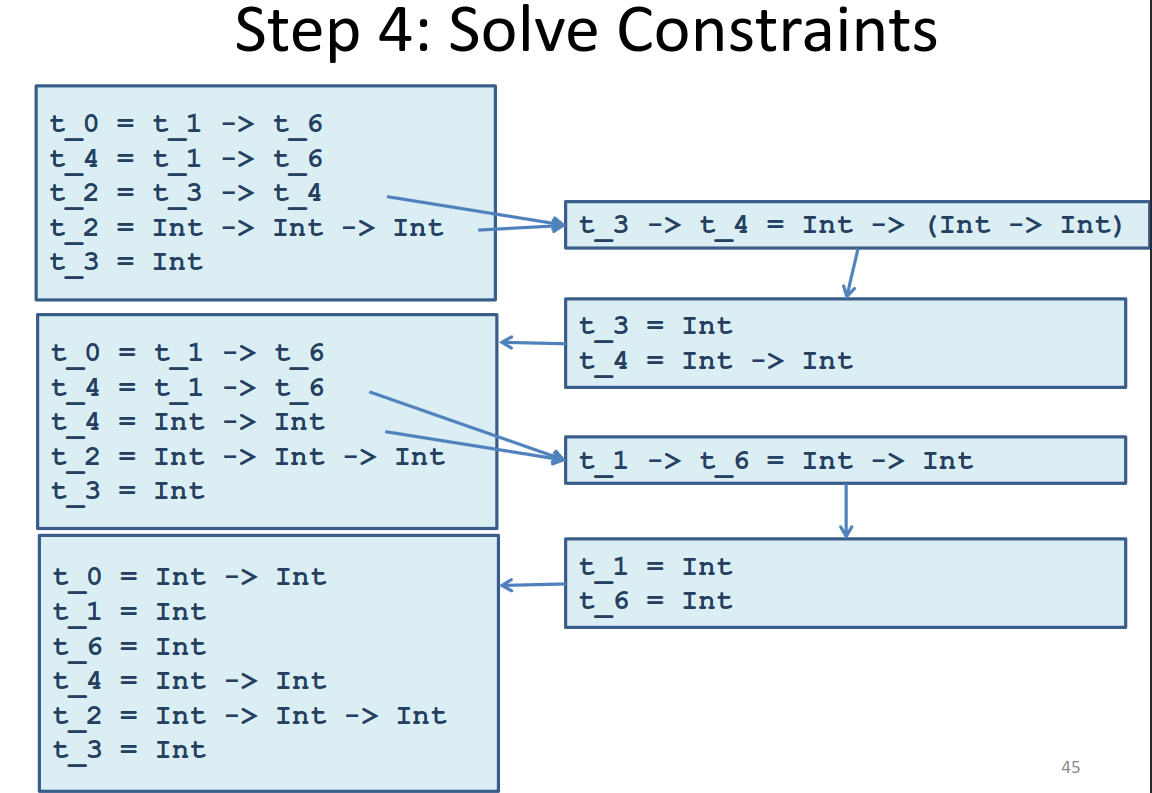
\includegraphics[width=0.4\columnwidth]{images/typeinference_step4.png}
   \label{fig:typeinference_step3_4}
\end{figure}

\begin{figure}[htbp]
   \centering
   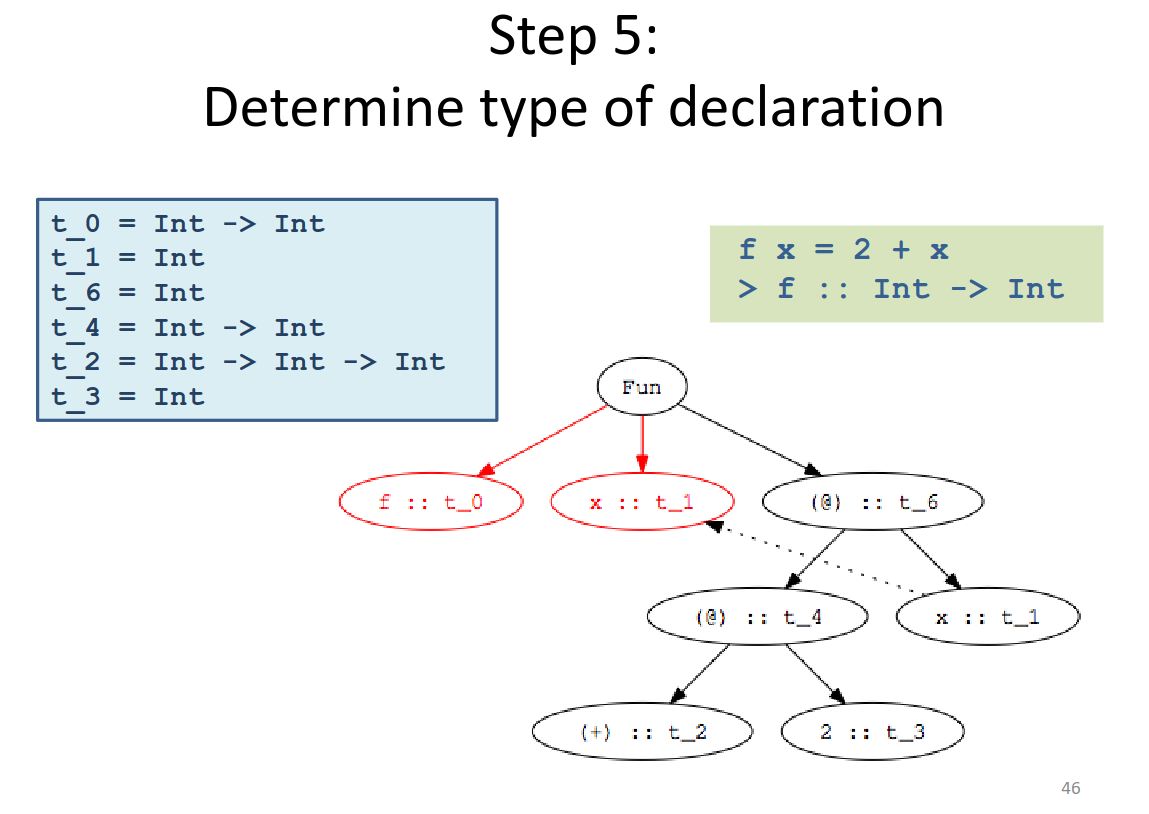
\includegraphics[width=0.4\columnwidth]{images/typeinference_step5.png}
   \label{fig:typeinference_step5}
\end{figure}
\newpage

\subsubsection{Steps summary}
\begin{enumerate}
   \item Parse program to build parse tree
   \begin{itemize}
      \item Each node is a function application \lstinline|@|, variable $x$, or constant
   \end{itemize}
   \item Assign type variables to nodes in tree
   \item Generate constraints:
   \begin{enumerate}
      \item From environment: constants (\lstinline|2|), built-in
      operators (\lstinline|+|), known functions (\lstinline|tail|).
      \item From shape of parse tree: e.g., application and
      abstraction nodes.
   \end{enumerate}
   \item Solve constraints using unification
   \item Determine types of top-level declarations
\end{enumerate}

\subsection{Polymorphism}

In general \textbf{unconstrained} type variables become \textbf{polymorphic types};
for instance, in the example below \lstinline|t_4| is unconstrained, hence we get a polymorphic type:
\begin{lstlisting}
   f g = g 2
   > f :: (Int -> t_4) -> t_4
\end{lstlisting}
\nl

For functions with multiple clauses, i.e. \textit{polymorphic datatypes},
for each clause a separate type is inferred, 
and then the resulting types are combined by adding constraints such as that all clauses have the same type.
In case of \textit{recursive calls}:
the function has same type as its definition.

\begin{lstlisting}
   append ([],r) = r
   append (x:xs, r) = x : append (xs, r)
\end{lstlisting}

\begin{enumerate}
   \item Infer type of each clause
   \begin{enumerate}
      \item First clause:
      \begin{lstlisting}
   > append :: ([t_1], t_2) -> t_2
      \end{lstlisting}
      \item Second clause:
      \begin{lstlisting}
   > append :: ([t_3], t_4) -> [t_3]
      \end{lstlisting}
   \end{enumerate}
   \item Combine by equating types of two clauses
   \begin{lstlisting}
   > append :: ([t_1], [t_1]) -> [t_1]
   \end{lstlisting}
\end{enumerate}

\subsection{Overloading}
In presence of \textbf{overloading} (\textit{Type Classes}), type inference infers a \textbf{qualified type} \lstinline|Q => T|
\begin{itemize}
   \item T is a Hindley Milner type, inferred as seen before
   \item Q is set of type class predicates, called a constraint
\end{itemize}
\begin{lstlisting}
   example :: Ord a => a -> [a] -> Bool
   example z xs = 
      case xs of
         [] -> False
         (y:ys) -> y > z || (y==z && ys == [z])
\end{lstlisting}

\begin{paracol}{2}
   \colfill
   In the example \textbf{Type} \lstinline|T| is \lstinline|a -> [a] -> Bool|
   while the \textbf{Constraint} \lstinline|Q| is \lstinline|{ Ord a, Eq a, Eq [a]}|.
   \lstinline|Q| later simplifies\footnote{According to some rules not discussed here} to \lstinline|Ord a|
   \colfill
   \switchcolumn

   \begin{itemize}
      \item \lstinline|Ord  a| because \lstinline|y>z|
      \item \lstinline|Eq a| because \lstinline|y==z|
      \item \lstinline|Eq [a]| because \lstinline|ys == [z]|
   \end{itemize}
\end{paracol}

\section{Type Constructors}
\textbf{Type Classes} are \textit{predicates} over \textit{types},
while \textbf{[Type] Constructor Classes} are \textit{predicates} over \textit{type constructors}.

For example, consider three versions of the \lstinline|map| function (implementation is omitted): the basic one for lists, one for trees and one for \lstinline|Maybe|.
\begin{lstlisting}
   map :: (a -> b) -> [a] -> [b]
   mapTree :: (a -> b) -> Tree a -> Tree b
   mapMaybe :: (a -> b) -> Maybe a -> Maybe b
\end{lstlisting}
They all share the same structure, thus they can all be written as
\begin{lstlisting}
   fmap:: (a -> b) -> g a -> g b
\end{lstlisting}
where \lstinline|g| is a function from \textit{types to types}, i.e.
a \textbf{type constructor};
it is:
\lstinline|[-]| for lists, \lstinline|Tree| for trees, and \lstinline|Maybe| for options.

\subsection{\texttt{Functor}}
This pattern can be captured in a constructor
class \lstinline|Functor|. 
A \textbf{constructor class} is simply a type class where
the predicate is over a type constructors rather
than on a type:
\begin{lstlisting}
   class Functor g where
      fmap :: (a -> b) -> g a -> g b
\end{lstlisting}

Compare with the definition of a \textit{standard type class}:
\begin{lstlisting}
   class Eq a where
      (==) :: a -> a -> Bool
\end{lstlisting}

So, wrapping up, we can instantiate \lstinline|Functor| on all three data structures,
and then simply use the \textit{overloaded} symbol \lstinline|fmap|, instead of \lstinline|map|, \lstinline|mapTree| and \lstinline|mapMaybe|.
\begin{lstlisting}
   class Functor f where
      fmap :: (a -> b) -> f a -> f b
   instance Functor [] where // [] is an instance of Functor
      fmap f [] = []
      fmap f (x:xs) = f x : fmap f xs
   instance Functor Tree where // Tree is an instance of Functor
      fmap f (Leaf x) = Leaf (f x)
      fmap f (Node(t1,t2)) = Node(fmap f t1, fmap f t2)
   instance Functor Maybe where // Maybe is an instance of Functor
      fmap f (Just s) = Just(f s)
      fmap f Nothing = Nothing
\end{lstlisting}

\note{Alternatively we could also write \lstinline|fmap = map|, \lstinline|fmap = mapTree|, fmap = \lstinline|mapMaybe|}

The following is an example on how to use the obtained fmap:
\begin{lstlisting}
   ghci> fmap (\x->x+1) [1,2,3]
   [2,3,4]
   it :: [Integer]
   ghci> fmap (\x->x+1) (Node(Leaf 1, Leaf 2))
   Node (Leaf 2,Leaf 3)
   it :: Tree Integer
   ghci> fmap (\x->x+1) (Just 1)
   Just 2
   it :: Maybe Integer
\end{lstlisting}